\graphicspath{ {imgs/} }
\documentclass[main.tex]{subfiles}
\begin{appendices}
\chapter{Software}
\label{app:software}
\section{Python}
\label{appendix:py}
Python is a multi-purpose language, which means that no specific coding paradigma is imposed on the user, but one can use scripting as well as object oriented design alike. This allows for a very flexible style of programming which was used in this project for writing little tools that help with the data preprocessing as well as more complex code for the learning pipeline and the analysis of the network. Python is also widely used by the machine learning community which makes it easier to look up code examples and questions on forums like \href{https://stackoverflow.com/}{Stackoverflow}. The specific version used in this thesis is 3.6 and all used packages are downloaded via pip or conda. The dependencies are listed in the file ``act-env.yml" and can be installed with it as well.

\section{Oracle Grid Engine}
\label{appendix:oge}
Our institute uses the work stations and additional hardware resources in form of a grid computing system that is managed by the Oracle grid engine (formerly known as Sun Grid Engine). The software manages the distribution of jobs to the nodes in the cluster, based on availability and resource requirements. The following bash script \ref{code:cluster} is used in the learning process of the network. It defines the name of the job and the necessary memory that should be available on the machines.

\begin{minipage}[t]{0.9\textwidth}
\begin{lstlisting}[language=bash, caption={The code for calling the learning script. The parameters in the beginning are the information for the Oracle Grid Engine.}, captionpos=b]
#!/bin/bash
#$ -N acts
#$ -l mem=128G
#$ -pe default 8
#$ -j y
#$ -v TESTNAME,WD,LOG_PATH

export LD_LIBRARY_PATH=$HOME/.local/cuda/lib64/:$LD_LIBRARY_PATH
export LIBRARY_PATH=$HOME/.local/cuda/lib64/:$LIBRARY_PATH
export CPATH=$HOME/.local/cuda/include:$CPATH
export PATH="/net/store/cv/projects/software/conda/bin:${PATH}"

. activate acts-cpu

python3 $WD/acts/src/learn.py \
        -d /net/store/cv/projects/datasets/image/pub/LIDC-IDRI/ \
        -l $LOG_PATH \
        -e 2000 \
        -s 1 \
        -b 5 \
        -n $LOG_PATH \
        -t $TESTNAME \
        -p 3000
\end{lstlisting}
\label{code:cluster}
\end{minipage}

No machine with less memory is considered by the distributor as an execution host for this job. If the memory is set too low for the job, it can not complete the task and fails during execution since no more than the requested memory can be allocated dynamically during run time. It is also defined how many cores should be used on the host machine to run the job in parallel. The job can be directly executed via the command line or with a script (which makes more sense if one plans to run the grid job multiple times). The command used for this operation is \emph{qsub}. Since the grid engine works with a concept of different queues it is possible to submit the job also just to specific queues, where one has the maximum execution time for example.

\begin{minipage}[t]{0.9\textwidth}
\begin{lstlisting}[language=bash, caption={The code for submitting the script to the scheduler.}, captionpos=b]
#!/bin/bash
export TESTNAME=Huang_no_scaling_50x50
export LOG_PATH=/net/store/cv/projects/tmp/asuckro/logs/acts_$(date +%Y-%m-%dT%H-%M)_$TESTNAME

mkdir -p $LOG_PATH

qsub -q all.q -o $LOG_PATH/grid.out runActs.sge
\end{lstlisting}
\end{minipage}

All jobs are only allowed for a specified maximal amount of time depending on the users setting and the queue the job is transmitted to. All outputs to the console are logged in a file that can be specified with the '-o' variable. 

\section{Tensorflow}
\label{appendix:tf}
Tensorflow is a software library developed by Google Brain that aids the development of machine learning applications by expressing computations as a graph and taking care of the underlying optimization and execution. The version used in this thesis was 1.3.0. The approach of the framework is applicable to many computational tasks apart from neural networks as long as they can be formalized in a graph, but many of the higher level functions in the framework deal with neural networks. Tensorflow is usable via API's for Python, C++, Haskell, Java, Go, and Rust. Third party packages are available for C\#, Julia, R, and Scala. Solving a problem with Tensorflow includes roughly two steps: first one needs to define a graph. A graph in Tensorflow is comprised of nodes, which are either variables (called Placeholders) or operations on those. The convolutional neural network in this thesis is defined like this: placeholders have been created for the lung patches that should be learned on, their respective labels and the phase of the learning (a boolean used for batchnormalization). Those are fed into basic transformation functions that handle the randomized flipping and rotating. The output of this function is fed into some summaries and further piped through the network. The covolutional layers have been scoped and encapsulated to own functions. The result of the dense layers is used to calculate the error that is used for the backpropagation learning in combination with the gradients. The complete structure can be seen in Figure~\ref{fig:tb}. The completed graph can now be executed in a Tensorflow session. In the session the placeholders are filled with data and a loop is used train the network for a specified number of epochs. Tensorflow only calculates the graph up to the point necessary for the queried parameter. So one can easily just ask for the prediction and skip the weight adaptation step as necessary for the analysis.

\begin{figure}[ht]
\centering
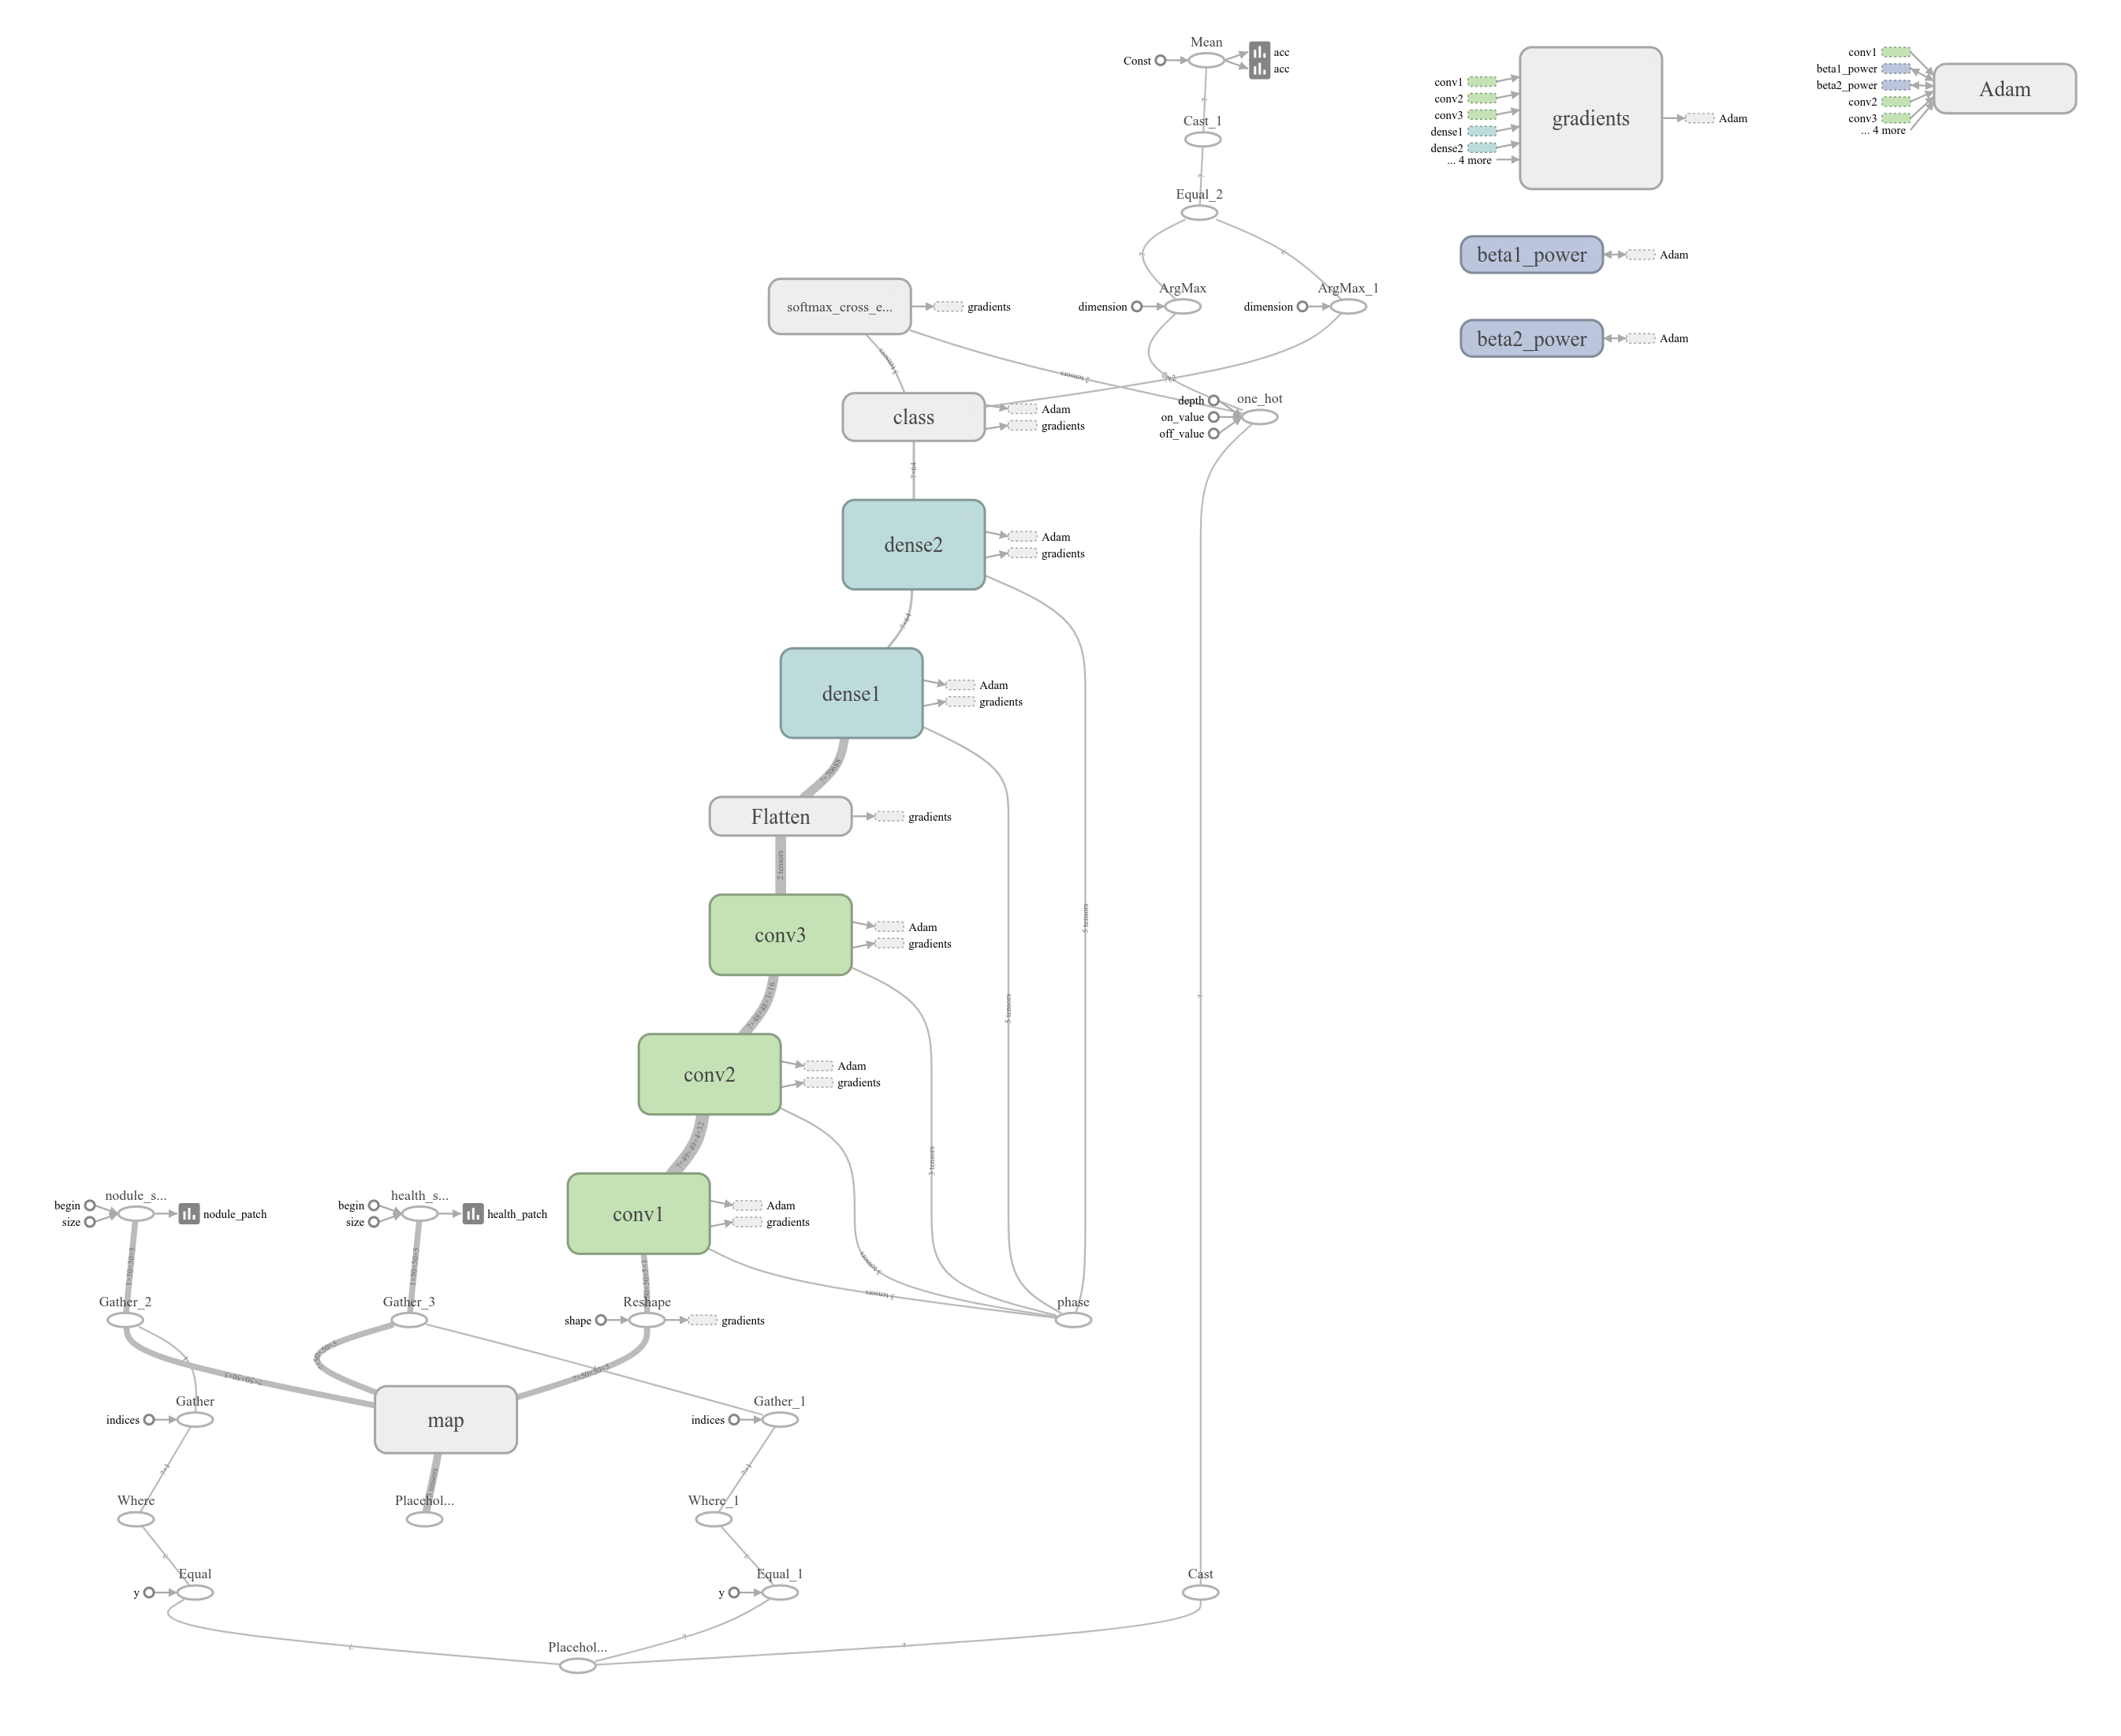
\includegraphics[scale=0.25]{tensorboard.png}
\caption{The graph of the model that was generated for this thesis. Scoping of the different layers help a lot to encapsulate similar behavior. The Placeholders do not only flow through the network but are used to generate summaries and reports.}
\label{fig:tb}
\end{figure}



\chapter{Data}
\label{appendix:data}
\section{LIDC-IDRI Dataset}
\label{appendix:lidc}
The database as it is available now is the result of a long process that began in April 2000. The National Cancer Institute (NCI) - the U.S. federal government's principal agency for cancer research and training submitted RFAs to create guidelines of how such a combined reference database could look like. The Lung Image Database Consortium (LIDC) was formed by the Weill Cornell Medical College, University of California, Los Angeles, University of Chicago, University of Iowa and University of Michigan in 2001. There task was to develop a web-accessible resource for CT scans with attached meta information (like the slice thickness, tube current and other technical specifications as well as patient information) and nodule information based on expert knowledge. The initiative was further advanced in 2004 by the Foundation for the National Institutes of Health (FNIH) which founded the Image Database Resource Initiative (IDRI). They brought two additional medical centers (MD Anderson Cancer Center and Memorial Sloan-Kettering Cancer Center) and eight imaging companies (AGFA Healthcare, Carestream Health, Inc., Fuji Photo Film Co., GE Healthcare, iCAD, Inc., Philips Healthcare, Riverain Medical, and Siemens Medical Solutions) to the initiative. The new members contributed significantly to the whole database and since the process of data aquisition and annotation was streamlined to the previous recorded data the whole set is referred to as the LIDC-IDRI Database. It's aim is to further develop, improve and evaluate automated methods for lung cancer detection and diagnosis and it is comparable to other public datasets in the medical data community like the Digital Database for Screening Mammography (DDSM) which contains roughly 3000 mammograms - a pioneer in the field of public medical imaging datasets.

\section{CT Scanner Technology}
CT scanners cover a wide range of computed tomography devices, like positron emission tomography (PET) and single-photon emission computed tomography (SPECT), but most commonly refer to tube X-ray scanners. Those scanners work roughly like this: the object of interest (the patient) is placed in the center of the tube. A X-ray emitter rotates around the object and gives off radiation that pierces through the object and is reflected depending on the density of the materials the object is composed of. Those differences in X-ray absorption make it possible to separate bones, nodules and blood vessels later on in the analysis. The recorded 2D images are combined by a software to a 3D representation, which makes it often necessary that the patients hold very still, even holding their breath during a scanning session. 

\begin{figure}[ht]
\centering
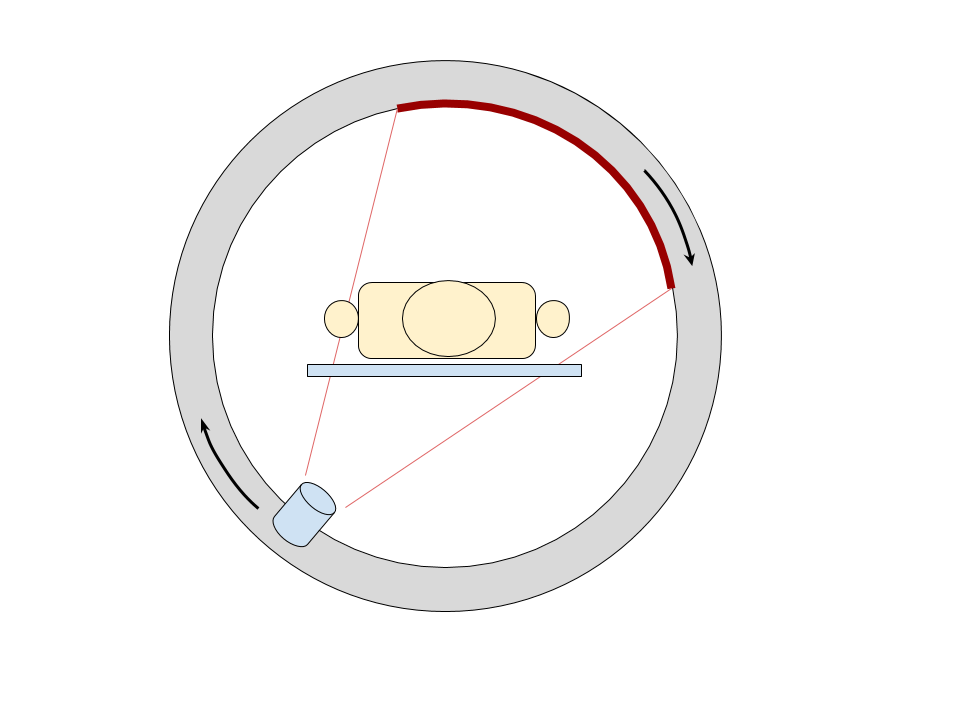
\includegraphics[scale=0.25]{ct_scanner.png}
\caption{This sketch illustrates the fundamental operation of a CT scanner. An emitter is rotating together with the sensor around the patient's body. The so recorded 2D images are used to reconstruct a 3D representation of the inner body.}
\label{fig:tb}
\end{figure}


\section{CT Specifications}
\label{appendix:scanner}
A range of scanner manufacturers and models was used to generate the data. The models and the number of samples they provided in the database are listed in the following table:

\begin{center}
\begin{tabular}{|||p{3,5cm}|p{3,5cm}|p{3,5cm}|p{3,5cm}|||} 
 \hline
 GE Medical Systems LightSpeed & Philips Brilliance & Siemens Definition, Emotion, Sensation & Toshiba Aquilion \\ [0.5ex] 
 \hline
 670 & 74 & 205 & 69 \\ [1ex] 
 \hline
\end{tabular}
\captionof{table}{The distribution of the 1018 samples among each CT scanner model. Vaules are taken from \cite{armato2011lung}}.
\end{center}

The tube peak potential energies used for scan acquisition were as follows: 120 kVp , 130 kVp , 135 kVp and 140 kVp. Tube current ranged from 40 to 627 mA (mean: 222.1 mA). 

The number of images per patient depend on the body size but also on the slice thickness which was 0.6 mm, 0.75 mm, 0.9 mm, 1.0 mm, 1.25 mm, 1.5 mm, 2.0 mm, 2.5 mm, 3.0 mm, 4.0 mm and 5.0 mm and the reconstruction interval that ranged from 0.45 to 5.0 mm (mean: 1.74 mm) \cite{armato2011lung}.

The number of pixels for each scan slice depends on the in plane resolution which ranged from 0.461 to 0.977 mm per pixel(mean: 0.688 mm). While the convolution kernels used for image reconstruction differ among manufacturers, these convolution kernels may be classified broadly as “soft” (67) math formula, “standard/nonenhancing” (n=560), “slightly enhancing” (n=264), and “overenhancing” (n=127) (in order of increasing spatial frequencies accentuated by each class).
\end{appendices}
